\section{Analysis}
\label{sec:analysis}
%(2 pages)

As noted previously, progress on knowledge base population has been slow and arduous.
Let's proceed with an analysis of submissions and evaluations thus far, with the motivation of identifying potential obstacles for system development. 

\paragraph{Data.}
We will make use of system submissions released as part of the TAC-KBP Slot Validation tracks in 2013, 2014 and 2015.

% TODO?
% Dataset statistics. -- number of documents, queries, submissions; heatmap of submission x query.
% Assume that systems by the same university are more similar and group by that axes?

\begin{figure*}
  \begin{subfigure}{0.49\textwidth}
  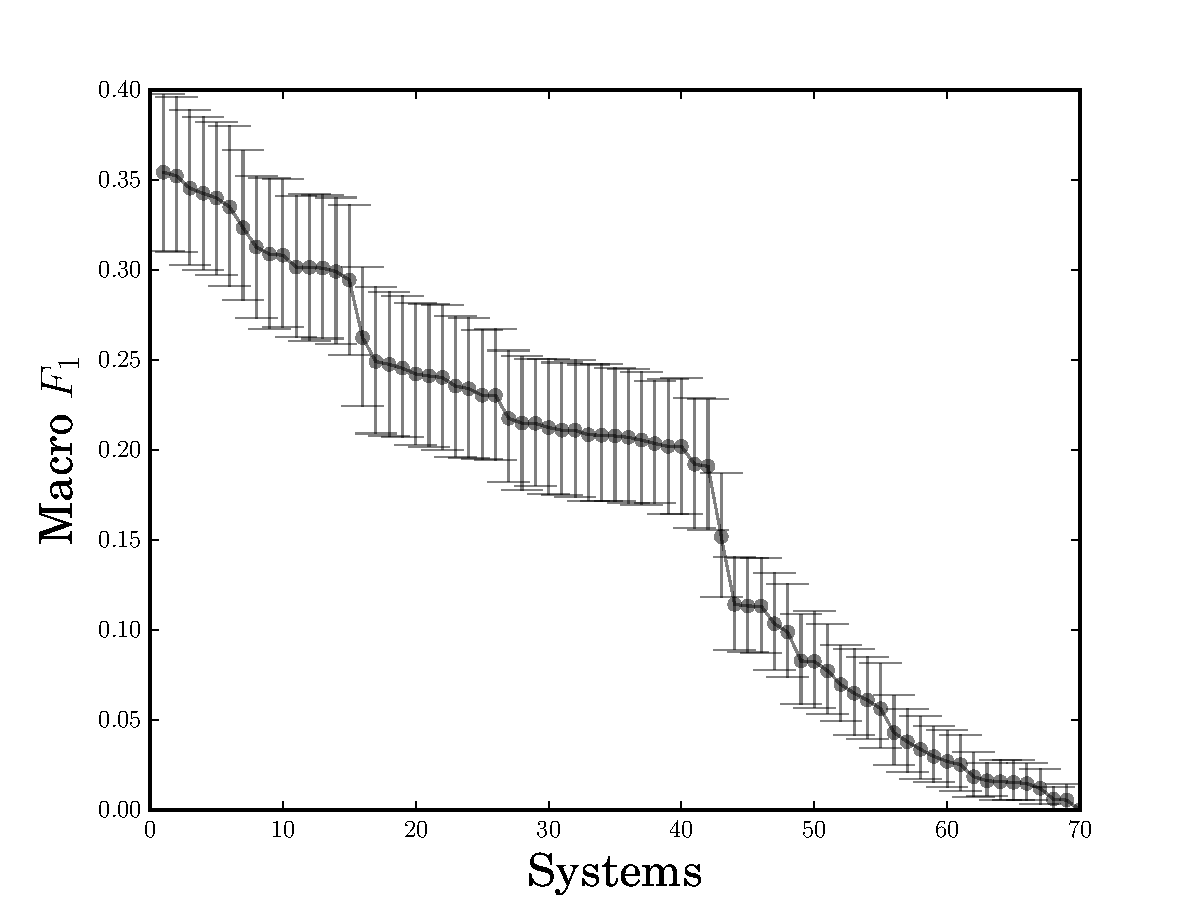
\includegraphics[width=\columnwidth]{figures/experiment1}
  \end{subfigure}
  \begin{subfigure}{0.49\textwidth}
  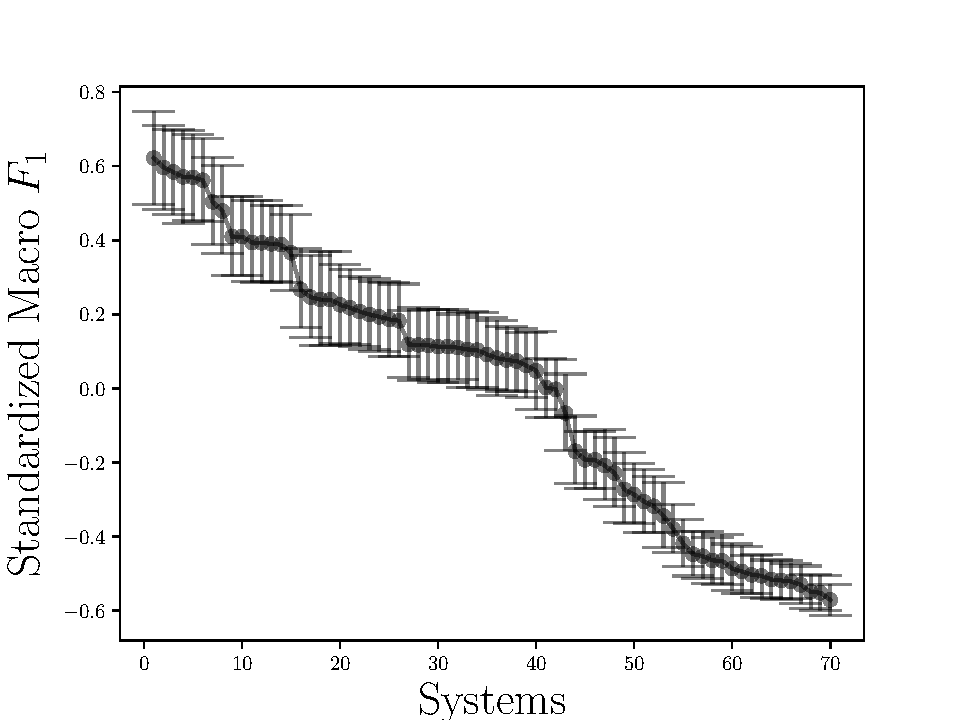
\includegraphics[width=\columnwidth]{figures/experiment3}
  \end{subfigure}
  \caption{}
\end{figure*}

\paragraph{How informative is macro/micro \fone{} as a metric?}
Most teams hill climb on a combination of micro and macro entity-level $\fone$ during development.
While \fone{} is a natural choice, it is possible for factors other than the system's intrinsic performance to have a disproportionate influence on its value.  
As a result, candidate developments may be erroneous regarded as favorable or unfavorable due to confounding factors. 


One natural confounding variable is the difficulty of query entities.
We can measure the effect of the query entity by analyzing the variation in topic-model scores.
Consider the linear model,
\begin{align*}
  X_{s,e} &= \mu 
    + \underbrace{\mu_{s} - \mu}_{\nu_{s}}
    + \underbrace{\mu_{e} - \mu}_{\nu_{e}}
    + \underbrace{X_{s,e} - \nu_{s} - \nu_{e} - \mu}_{\nu_{s,e}},
\end{align*}
where $\nu_{s}$, $\nu_{e}$ and $\nu_{s,e}$ capture the effect of the system $s$ and query entity $e$, and the residual.
Variance can also be decomposed as,
\begin{align*}
  \sigma^2(X_{s,e}) &= \sigma^2(\nu_s) + \sigma^2(\nu_e) + \sigma^2(\nu_{s,e}).
\end{align*}

\tableref{} shows the variance explained by different components for macro metrics. As we can see, almost twice as much of the variance is explained by the entity only as that of the system.
% Explain what the high q,e scores mean.
Another consequence is in confidence intervals.
Bad differentiation from pairwise scores.

\paragraph{A better metric: standardized \fone.}

$X'_{st} = \frac{X_{st} - \mu_t}{\sigma_t}$.

Another way of measuring this is by estimating how much data is required to. By reducing the variance, we require fewer entities. 

New graph.

% TODO: I wish we could give scroes for this.
% \subsection{Are we improving over time?}

\begin{figure}
  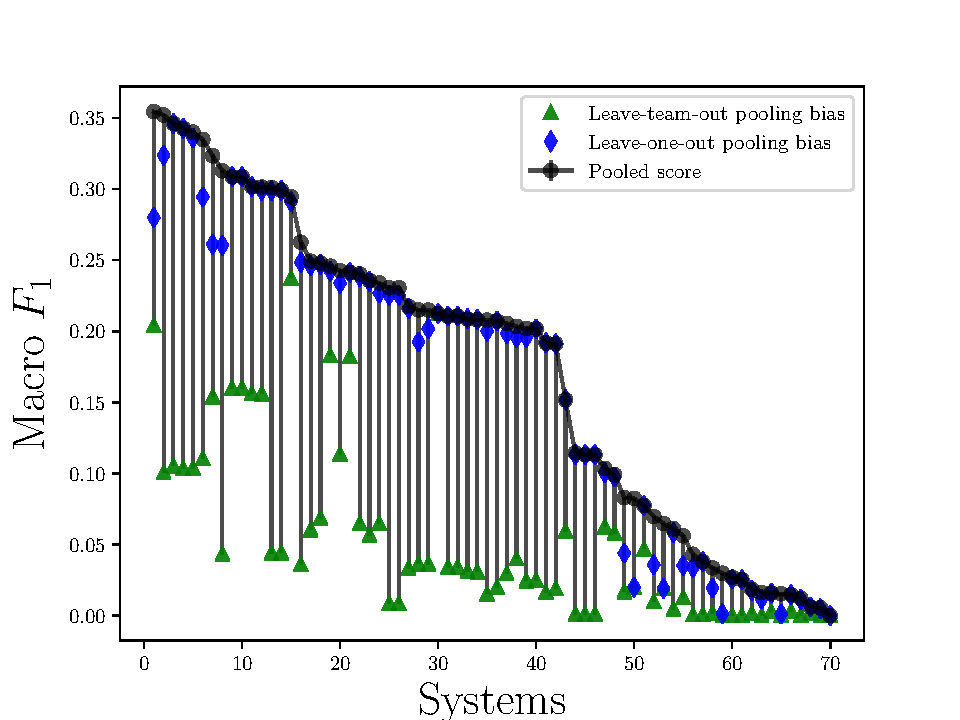
\includegraphics[width=\columnwidth]{figures/experiment2}
  \caption{Pooling bias.}
\end{figure}


\subsection{What is the effect of pooling?}

Define pooling bias. Statistical model used.
Significant!

If we increased the amount of data annotated, we may hopefully avoid pooling bias.
Expensive and perhaps regressive.
Next section, explore a new way.

